\chapter{Firmware}

\renewcommand{\kapitelautor}{Autor: Lucas Ullrich}

\section{Kamera}\label{Sec. Kamera}
Das Kameramodul besitzt viele unterschiedliche serielle Schnitstellen. Aufgrund der schnellen Datenübertragung wurde das Serial Peripheral Interface, kurz SPI, gewählt.\\
Mit dieser Schnitstelle ist es möglich mehrere Teilnehmer unabhängig von einander anzusprechen, das eignet sich vorallem für Erweiterungen der Hardware.\\
Die PIXY cmucam5 verlangt bei der Übertragung der Daten über SPI Synchonistationsbytes. Durch diese ist es der Kamera möglich zu überprüfen ob eine korrekte Datenübertragung stattfindet. Um ein word, also 16 Bit, an Daten zu übertragen müssen insgesamt drei Bytes unterschieden werden:
\begin{itemize}
\item 0x5a, um Daten von der Pixy zu lesen, das nachfolgende Byte hat keine Bedeutung
\item 0x5b, um Daten zu senden und zu lesen, das nachfolgende Byte enthält eine Bedeutung
\item 0x0, wird nachfolgend zu 0x versendet, kein weiterer Nutzen
\end{itemize}

Die Auswertung der Bilder gestaltet sich aufgrund der vergleichsweise großen Datenmenge etwas aufwändiger. Von der Kamera werden 50 Bilder pro Sekunde erfasst und können somit auch übertragen werden. Jedes einzelne Bild besteht aus einem word (0xaa55) um das neue Bild zu indizieren und 8 weiteren words, diese sind:
\begin{itemize}
\item Farbcode oder Objekt
\item Checksum
\item Objektnummer
\item X-Position
\item Y-Position
\item Breite
\item Höhe
\item Drehwinkel (Nur bei Farbcodes, sonst 0)
\end{itemize}

Für jedes Word muss hierbei ein neues Synchonisationsbyte gesendet werden.\\
Möchte man die Farbe der LED ändern, die mit der PIXY verbindbaren Servos ansteuern oder die Helligkeit der Kamera ändern so muss man 0x5b als Synchonisationsbyte senden, ansonsten 0x5a.

\begin{figure}[H]
\begin{centering}

\includegraphics[width = 60mm]{Bilder/Farbcode}
\par\end{centering}
\caption{Ein einfacher Farbcode}
\label{Farbcode}
\end{figure}

\subsection{Überprüfen der SPI-Schnittstelle}
Um sicher gehen zu können, dass die Schnittstelle auch korrekt funktioniert musste diese zuerst überprüft werden. Hierzu wird ein am Pin möglichst variierender Wert genommen (z.~B. 01010101) und mit einem Oszilloskop der tatsächliche Ausgang auf der entsprechenden Leitung überprüft.
\begin{figure}[H]
  \begin{centering}
    \subfigure[Großer Zeitbereich]{\includegraphics[width = 0.49\textwidth]{Bilder/SPI_gross}}
    \subfigure[Kleiner Zeitbereich]{\includegraphics[width = 0.49\textwidth]{Bilder/SPI_klein}}
  \end{centering}
  \caption{Ausgang der SPI-Schnittstelle}
  \label{SPI-Ausgang}
\end{figure}

\subsection{Erkennen eines Bildes}
Um ein Bild zu erkennen muss so lange nach der Startbedingung gesucht werden bis diese gefunden ist. Dabei können noch Daten von einem zuvor nicht vollständig ausgelesen Bild übertragen werden oder einfach 0 wenn das Senderegister der Kamera noch leer ist.

\lstset{language = C}
\begin{lstlisting}
while(frame == 0) {
    w = ExchangeSpi2char(PIXY_SYNC, DUMMY);
    if(lw == PIXY_FRAME_OBJ && w == PIXY_FRAME_OBJ) {
        frame = 1;
        obj_type = 0;
    } else if(lw == PIXY_FRAME_OBJ && w == PIXY_COLORCODE) {
        frame = 1;
        obj_type = 1;
    } else if(w == 0 && lw == 0){
        frame = 0;
    }
    lw = w;
    c++;
    if(c > 254) {
        return 0;	// Kommentar
    }
}
\end{lstlisting}

Dieser Programmablauf versucht 254 mal die Startbedingung eines neuen Bildes zu erfassen. Diese wird zusammen mit dem nächsten word genutzt um festzulegen ob ein Farbcode oder ein normales Objekt erkannt wurde. Sobald ein Bild und Farbcode/Objekt erkannt wurde wird die Schleife verlassen und das abspeichern der übrigen Daten beginnt. Wird nach 254 Veruchen nichts erkannt wird die gesamte zuvor aufgerufene Funktion verlassen, das verhindert ein ewiges festhängen in der Funktion.


Anhand dieser Messungen zeigt sich, dass die Kamera eindeutig nicht das zurückliefert was zuvor gesendet wurde sondern eigene Daten. Zusätzlich sind eindeutige Störungen im Signal erkennbar.

\subsection{Auswerten eines Bildes}
Um aus einem Bild nun auch die Flugdaten ermitteln zu können muss dieses entsprechend weiterverarbeitet werden. Dazu ist es nötig die unterschiedlichen Parameter der erkannten Objekte zuerst abzuspeichern.
\\Die Daten des betreffenden Objekts werden, sobald ein Bild erkannt wurde der Reihe nach eingelesen. Um die Korrektheit der Datenübertragung überprüfen zu können wird davor auch eine Checksumme übertragen. (siehe Kapitel \ref{Sec. Kamera} \nameref{Sec. Kamera})
\lstset{language = c}
\begin{lstlisting}
unsigned int checksum = ExchangeSpi2char(PIXY_SYNC, DUMMY);
afarben[c_obj].num =    ExchangeSpi2char(PIXY_SYNC, DUMMY);
afarben[c_obj].pos_x =  ExchangeSpi2char(PIXY_SYNC, DUMMY);
afarben[c_obj].pos_y =  ExchangeSpi2char(PIXY_SYNC, DUMMY);
afarben[c_obj].width =  ExchangeSpi2char(PIXY_SYNC, DUMMY);
afarben[c_obj].height = ExchangeSpi2char(PIXY_SYNC, DUMMY);
afarben[c_obj].angle =  ExchangeSpi2char(PIXY_SYNC, DUMMY);

if(ProofObject(des_obj, afarben[c_obj].num)) {
    LedSignalling(afarben[c_obj].pos_x, afarben[c_obj].pos_y);
}
\end{lstlisting}

Wurde das korrekte Objekt erkannt wurde zu Testzwecken mit LED's angezeigt wo es sich im Bildbereich befindet. Dies dient als erster Schritt zu einer Steuerung des Hexacopters anhand der Position eines Fabrcodes auf dem übertragenen Bild.
%\needspace{4cm}
\begin{figure}[H]
  \begin{centering}
    \includegraphics[width = 0.5\textwidth]{Bilder/Kameratest_LED}
  \par\end{centering}
  \caption{Anzeige der Farbcodeposition durch LED's}
  \label{LED-Anzeige}
\end{figure}

\subsection{Bestimmen des Flugmodus}
Um im Notfall manuell in das Geschehen eingreifen zu können soll der Hexacopter wahlweise Manuell oder automatisch gesteuert werden.
Der Flugmodus wird mit einem Schalter an der Fernsteuerung bestimmt. Dieser veranlasst den Empfänger dazu einen Puls mit einer Länge zwischen 1095 µs und 1896 µs auszugeben. Das Signal ist alle 20 ms periodisch wiederkehrend und besitzt 3 Signalwerte:

\begin{figure}[H]
\subfigure[Mode0]{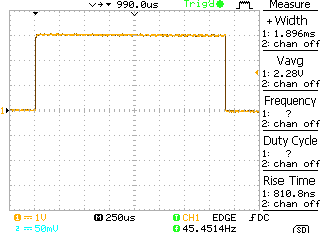
\includegraphics[width = 0.32\textwidth]{Bilder/Mode0}}
\subfigure[Mode1]{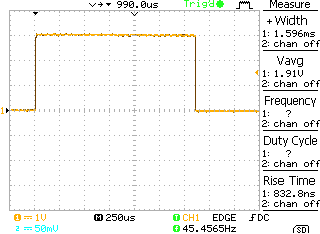
\includegraphics[width = 0.32\textwidth]{Bilder/Mode1}}
\subfigure[Mode2]{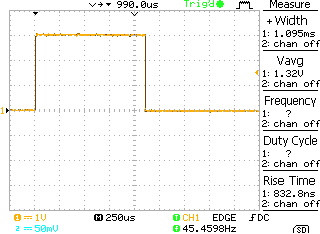
\includegraphics[width = 0.32\textwidth]{Bilder/Mode2}}
\caption{Signale des U-Pins}
\label{U-Signale}
\end{figure}
Den unterschiedlichen Signalen werden unterschiedliche Flugmodi zugeordnet. So entsprechen die zwei kürzeren Impulse (1095 µs und 1596 µs) einem manuellen Flug und der lange Impuls (1896 µs) einem autonomen Flug.
Der Impuls wird am Micro Controller durch einen 16-Bit Timer und dessen Gate-Anschluss ausgewertet.
Die Signale um den Hexacopter zu steuern werden durch einen Multiplexer zu dem Flightcontroller geleitet, abhängig vom Flugmodus werden die Steuerbefehle des 2,4 GHz Empfängers oder jene des Micro Controllers genutzt.

\lstset{language = c}
\begin{lstlisting}
unsigned int Fkt_CalcTime(void) {
    unsigned int time_pulse = TMR3H;
    time_pulse <<= 8;
    time_pulse |= TMR3L;
    TMR3H = 0;
    TMR3L = 0;
    NOP();
    return time_pulse;
}

$\textcolor{blue}{bit}$ Fkt_ModeCheck(void) {
    unsigned int time = Fkt_CalcTime();
    if(time < GEAR_TIME){
        LED = 0;
        return 0;
    }else if(time >= GEAR_TIME) {
        LED = 1;
        return 1;
    }
    NOP();
}
\end{lstlisting}

\section{Aufgetretene Fehler}
Während dem ersten vollständigem Systemtest trat das Problem auf, dass der Mikroprozessor scheinbar einen falschen Wert beim bestimmen der Flugmodus einliest. Der vorhandene Wert war jenseits von 60.000 im Timer-Register, bei den vorhandenen Einstellungen also \ca eine Impulsdauer von 15 ms. Bei einem Impuls der zwischen 1 und 2 ms lang sein sollte also viel zu viel.
Durch dieses Problem war natürlich auch der Flugmodus nicht mehr bestimmbar, also der Teil der alleine bereits funktionstüchtig war funktionierte nun nicht mehr. Nach einigen Messungen konnte festgestellt werden, dass ebenso viel zu wenige Messungen der Flughöhe, also mit dem Ultraschall-Sensor stattfanden.

Erst ein Test im Simulator brachte die Auflösung: Sobald das Echo des Ultraschallsensors beim PIC angekommen war und anschließend der Gear-Pin, also jener auf dem das Signal für den Flugmodus ankommt, den nächsten Impuls empfing dauerte es ausgesprochen lang bis der Simulator den an der Auswertung des Flugmodus gesetzten Breakpoint erreichte.

Das Problem schien erst einmal gefunden: der Mikroprozessor braucht viel zu lang für die gesamte Auswertung. Einer kurzen Nachrechnung zufolge kommen \ca 8 Impulse an bevor der Mikroprozessor erneut ein Signal verarbeitet.
Die einzig mögliche Lösung ist eine umstrukturierung des Programmes. Es wird nun besonders auf die empfangenen Impulse am Gear-Pin als auch auf die Ausgabe der Signale geachtet. Dies muss nämlich zwingend im 20 ms Rxthmus geschehen.
Die Auswertung der Flughöhe und der Kameradaten bekommt nun eine geringere Priorität und wird in der verbleibenden Zeit zwischen den vom Gear-Pin ausgelösten Interrupst durchgeführt. Dabei ist es nicht wichtig wenn nicht alle 20 ms eine Auswertung und damit einhergehend eine Änderung der Steuerpulse folgt. Eine Auswertung dieser 10 mal pro Sekunde ist immer noch vollkommen ausreichend.

Die Ausgabe der Impulse findet nun mithilfe von Interrupts des Compare Moduls und dem Timer 1 statt. So wird die Interrupt Subroutine nicht unnötig belastet und es kann dennoch jederzeit die entsprechende Ausgabe getätigt werden.
